\subsection{Asynchronous Kalman Filter}
\label{subsec:Kalman}


\begin{frame}{Asynchronous Kalman Filter - Introduction}
    \bit[label=\raisebox{0.25ex}{\tiny$\bullet$}]
        \item State estimator needed
        \vspace{5mm}
        \item Combine model \& measurement
        \vspace{5mm}
        \item Combine measurements
        \vspace{5mm}
        \item Controller vs measurement rate
    \eit
    		
\end{frame}


\begin{frame}{General working principle}

    \begin{figure}[h]
    \centering
    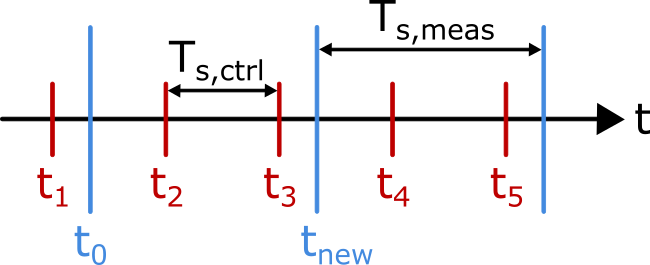
\includegraphics[width=10cm]{Figures/Kalman_general.png}
    \caption{General time schedule of input and measurement time stamps.}
    \label{fig:kalman_gen}
    \end{figure}
    		
\end{frame}